%!TEX root = these.tex

\chapter[La Réalité Virtuelle et la Biologie Moléculaire : usages, enjeux et perspectives]{La Réalité Virtuelle et la Biologie Moléculaire : usages, enjeux et perspectives}
\label{Sec:RV}
\minitoc
\cleardoublepage

%% Commentaire : la commande \texorpdfstring permet de déclarer un titre de
%% chapitre (ou section, sous-section) alternatif en texte seul, si besoin, qui
%% est utilisé par hyperref pour fabriquer un menu dans les fichiers compilés

%\chapter{\texorpdfstring{Contrôle gestuel de l'articulation}{Contrôle gestuel de l'articulation}}
%% Commentaire : la commande \texorpdfstring permet de déclarer un titre de
%% chapitre (ou section, sous-section) alternatif en texte seul, si besoin, qui
%% est utilisé par hyperref pour fabriquer un menu dans les fichiers compilés

%Exemple de notation qui sera reprise dans l'index : soit $\Q$\index{Q@$\Q$} le corps des nombres rationnels.


%Comme cela est le cas pour les outils de modélisation moléculaire, il est important d'amener les outils de visualisation à s'intégrer aux efforts de développement reflétés dans les technologies de pointe développées ces 10 dernières années. La démocratisation de ces dernières va ouvrir de nouvelles habitudes d'utilisation qui doivent être anticipées, que ce soit au sein des processus d'enseignement, de recherche ou bien de développement. Parmi les nouvelles technologies possédant un impact potentiel fort sur la biologie structurale, nous avons vu que la \textbf{Réalité Virtuelle} (RV) est un candidat idéal pour répondre à certaines des problématiques évoquées dans le chapitre précédent (voir section \ref{limits_persp_bio_struct}). Les investissements dans ce domaine sont conséquents et le fleurissement des projets de casques de RV par les plus grandes compagnies internationales de haute technologie (Facebook/Occulus, Samsung Gear VR, HTC Vive, Morpheus de Sony, etc.) au cours de ces derniers mois est la preuve d'un engouement général pour ces nouvelles technologies.


Les contributions de la Réalité Virtuelle (RV) pour résoudre des problématiques industrielles et scientifiques sont depuis quelques années de plus en plus nombreuses. Cet essor peut être expliqué par deux facteurs principaux : (1) la démocratisation des dispositifs de visualisation et d'interaction issus de la réalité virtuelle et augmentée et (2) l'apport de la 3d pour observer et manipuler des objets massifs complexes intrinsèquement tridimensionnels. Le besoin conjoint de mieux percevoir et de manipuler les objets tridimensionnels que constituent les structures moléculaires, a abouti à une appropriation assez rapide de techniques de RV comme la stéréoscopie par la communauté de biologie moléculaire. Dans ce chapitre, après quelques définitions nous décrirons plus en détail les apports de la RV pour la biologie structurale, en particulier en terme de modélisation et de simulation moléculaire.

\section{La Réalité Virtuelle} \label{RV_science}

%La RV, grâce à sa capacité à créer un monde artificiel où les informations peuvent être mêlées entre elles, tout en gardant leur signification, est tout adaptée pour répondre au défi de l'optimisation des processus d'analyses.

Plusieurs définitions de la Réalité Virtuelle ont été proposées depuis son émergence dans les années 90. Sherman et Craig définissent la RV comme le fait d'être immergé dans un monde virtuel interactif \cite{sherman2002understanding}. Brooks formule cette définition de façon presque similaire en disant que la RV est une expérience où l'utilisateur est efficacement immergé dans un monde virtuel réactif \cite{brooks1999s}. De façon légèrement différente, Burdea décrit la RV comme une simulation dans laquelle les graphismes générés par informatique sont utilisés pour créer un monde au rendu réaliste qui n'est pas statique, en répondant aux sollicitations de l'utilisateur \cite{burdea2003virtual}. On retrouve dans ces définitions les trois piliers qui définissent la RV selon Heim : Immersion, Interaction, Information \cite{heim1998virtual}. Bien qu'il soit difficile d'extraire une définition simple et unique de la RV, l'idée principale est bien de mettre l'utilisateur au centre d'un environnement dynamique et réactif, créé artificiellement et qui viendra se supplanter au monde réel le temps de l'expérience. Cette définition est très proche de la définition de la RV que nous considérons au sein de l'équipe VENISE du LIMSI-CNRS \cite{bourdot_patrick_reconstruction_2002}:

\textit{La Réalité Virtuelle vise à mettre au point des systèmes informatiques qui donnent à l'humain la capacité de percevoir et d’interagir de façon multi-sensori-motrice avec des données numériques ou mondes virtuels. Quand en plus, ces données numériques intègrent une virtualisation d’une partie de l’univers réel et permettent ainsi de gérer des interactions entre des objets réels et des objets virtuels, on parle alors de Réalité Augmentée, voire de Réalité Mixte.
}

\subsection{Immersion}

L'immersion se caractérise par la mise en place de techniques donnant à percevoir à l'utilisateur des retours sensoriels artificiels suffisamment réalistes et écologiques d'un point de vue perceptif pour lui donner l'illusion d'être immergé dans un monde virtuel. L'interaction constitue une dimension primordiale de ce réalisme, puisque le rendu visuel doit être dynamique en fonction de la direction du regard et de la position de l'utilisateur, condition minimum pour assurer la sensation d'immersion en mimant la perception écologique du monde réel. 

Les informations présentées dans la scène virtuelle durant l'expérience  immersive peuvent être adressées à plusieurs canaux sensoriels, majoritairement les canaux visuel et auditif, mais peuvent aussi mobiliser d'autre sens. De la richesse de ces retours et de la qualité d'intégration dépendra la qualité et le degré d'immersion de l'utilisateur. Bowman et McMahan notent qu'il n'est cependant pas nécessaire de gérer l'ensemble des sollicitations sensorielles d'un utilisateur pour assurer une sensation d'immersion  \cite{bowman_virtual_2007}. Dans cette même étude, les auteurs proposent un découpage de l'immersion en plusieurs composants, mettant en avant le fait qu'une immersion n'est ni complètement absente, ni parfaite, mais qu'elle peut être considérée au sein un continuum. L'immersion, concept essentiellement perceptif, induit chez l'utilisateur le sentiment d'être présent et incarné dans le monde virtuel, appelé sentiment de présence. Par opposition à l'immersion qui provient de la manipulation des sens de l'utilisateur avec une dimension essentiellement perceptive, la présence est un concept essentiellement cognitif puisqu'il s'agit d'un état de conscience dans lequel le sujet a le sentiment d'évoluer dans le monde virtuel et d'y être l'acteur. Bowman et McMahan mettent également en avant des applications de RV où le concept de présence de l'utilisateur n'est pas central. Parmi ces applications, la visualisation de données scientifiques, qui nous intéresse dans notre étude, met en effet davantage l'accent sur le contenu que sur la qualité d'immersion de l'utilisateur dans son monde virtuel.

Il est important de faire la distinction entre l'immersion perceptive et l'immersion cognitive. Alors que l'immersion perceptive est le résultat de la sollicitation sensorielle d'un individu pour qu'il se sente immergé, l'immersion cognitive se base principalement sur l'aspect psychologique de l'individu. 
L'immersion perceptive est donc plus directe et s'appuie sur un rapport étroit avec la réalité puisque des stimuli réels pourront être utilisés pour piéger les sens d'un individu en immersion. L'immersion cognitive s'intéressera par contre à l'imagination et à la représentation mentale de l'utilisateur qui provoque l'état d'immersion. Ces deux facettes de l'immersion sont présentes à des degrés différents suivant les applications mais sont rarement ni complètement présentes ni complètement absentes. L'immersion cognitive tend à prendre une place de plus en plus importante au sein des nouvelles technologies. Les vidéos 360 degrés récemment rendues très facilement accessibles via la plateforme Youtube sont un exemple de moyen d'immersion à la fois cognitif et immersif. En effet, l'utilisateur  manipule son smartphone doté d'un accéléromètre et/ou d'un gyroscope, qui fait office de fenêtre de visualisation sur le monde virtuel, dont il peut changer la position et l'orientation pour observer un monde virtuel tout autour de lui. Il y a alors construction d'une carte mentale de ce monde virtuel, à partir d'une perception parcellaire de ce monde virtuel à travers cette fenêtre dynamiquement contrôlée par le sujet.

\subsubsection{Visuelle}\label{immersion_visuelle}

Les interfaces visuelles sont de loin les plus utilisées pour l'immersion et bien que d'autres interfaces soient également utilisées dans des cas ponctuels, elles le sont rarement sans couplage à des interfaces visuelles. Ces dernières stimulent le sens de la vue de l'utilisateur et doivent parvenir à fournir un confort visuel le plus proche possible des conditions écologiques.

\myparagraph{Stéréoscopie ou rendu 3d} \label{stereo_3d}

On ne peut évoquer les interfaces visuelles immersives sans s'arrêter sur le concept de stéréoscopie, participant à la qualité de l'immersion. La stéréoscopie se caractérise par la génération de deux images distinctes, une pour chaque œil, avec un décalage de point de vue correspondant à l'image que verrait l'œil si le second était fermé. Lorsque chaque image est présentée à l'œil correspondant, le cerveau traite ces images afin de faire percevoir de la profondeur et du relief dans la scène observée. Ces images sont restituées par un écran ou un projecteur, mais doivent ensuite être séparées afin d'atteindre indépendamment les deux yeux. Cette séparation peut se faire soit de façon \textit{active}, soit de façon \textit{passive}. Lorsque la séparation est \textit{active}, on occulte la vision des deux yeux de manière alternée et à haute fréquence. Une succession d'images alternant le point de vue de l'œil droit et le point de vue de l'œil gauche est ainsi diffusée. Il est donc nécessaire d'afficher la bonne image pour le bon œil au moment où celui-ci n'est pas occulté, impliquant donc une forte synchronisation entre le générateur d'images et la lunette à occultation utilisée.
Dans le cas d'une séparation \textit{passive} des images, on utilise un filtre polarisant à la fois sur les écrans et les lunettes. Les deux images sont ici affichées en même temps mais selon deux polarités différentes ce qui permet leur distinction par le filtre polarisé correspondant, un différent à chaque œil. Une polarité basée sur les couleurs donnera lieu par exemple à la diffusion d'une image rouge pour l'œil gauche, une image bleue pour l'œil droit qui seront toutes deux superposées, le filtre bleu ou rouge des deux verres de lunettes permettant de faire la séparation.

\myparagraph{Vision adaptative grâce au \textit{tracking}} \label{visu_adaptative}

La \textbf{stéréoscopie adaptative} désigne la technique permettant de faire varier un rendu graphique 3d en fonction de la position et de l'orientation de l'utilisateur. Elle se base principalement sur la capture de cette position de façon instantanée et continue. Chaque nouvelle position de l'utilisateur déclenche ainsi un changement dans le contenu 3d affiché permettant de retranscrire le changement visuel attendu, conséquence du mouvement de l'utilisateur.

Parmi les dispositifs permettant de récupérer les positions de la tête ou du corps de l'utilisateur, le \textbf{tracking optique} est l'un des plus usités. Il fonctionne au moyen de caméras infrarouges et de marqueurs réfléchissants (voir Figure \ref{Fig:ir-tracking}). Des motifs de marqueurs vont servir de cibles pour les caméras infrarouges qui vont opérer une triangulation afin d'en extraire leur position. Chaque motif différent peut être associé à un objet particulier, une partie du corps ou un dispositif d'interaction. Le suivi de la tête est particulièrement utile dans les environnements immersifs puisqu'il permet de connaître la direction exacte du regard de l'utilisateur au sein du monde virtuel. Grâce à cela, les ordinateurs responsables du rendu graphique peuvent adapter les images affichées sur les écrans pour qu'elle corresponde au point de vue de l'utilisateur dans le monde virtuel.

\begin{figure}
  \centering
  {\includegraphics[width=.65\linewidth]{./figures/ch2/IR-tracking}}
    \caption[Schéma simplifié d'un système de tracking optique.]{{\it Schéma simplifié d'un système de tracking optique ART basé sur des signaux infrarouges lancés par des caméras et se reflétant sur des marqueurs spécifiques. La configuration spatiale des marqueurs est reconnue par le PC et la position associée est calculée à partir des intersections de rayons infrarouges reflétés.}}
  \label{Fig:ir-tracking}
  \hspace{0.3cm}
\end{figure}

Le tracking optique demande la mise en place d'un système encombrant et spécifique, pour des conditions de luminosité et d'espace de travail limitées, et n'est parfois donc pas envisageable. il est alors possible d'utiliser la vision adaptative grâce à des instruments de mesures embarqués dans un dispositif mobile porté par l'utilisateur. Ces derniers ne permettent pas un suivi absolu de la position de l'utilisateur dans l'espace mais un suivi relatif de l'orientation de son regard. Les \textbf{gyroscopes}, présents dans l'intégralité des smartphones par exemple, permettent cette interprétation et, à la manière du tracking optique, envoient à l'application les informations d'orientation afin que le rendu graphique soit adapté.

Ces deux approches demandent une certaine efficacité dans la rapidité d'interprétation des positions/orientations de l'utilisateur et du calcul graphique 3d afin de réduire au maximum le temps de latence entre un mouvement et son effet sur le rendu de la scène.

Nous avons vu les principales techniques permettant de générer de la stéréoscopie 3d, statiques ou adaptatives, intéressons-nous maintenant aux dispositifs permettant de diffuser ces images.

\myparagraph{Dispositifs} \label{dispositifs_RV}


Il est difficile de décrire la RV sans décrire les dispositifs qui lui servent de support. Conçus pour solliciter l'ensemble des canaux sensori-moteurs de l'homme, ces dispositifs doivent permettre à l'utilisateur de percevoir le monde virtuel dans lequel il évolue de la manière la plus nette et claire possible afin qu'il y interagisse efficacement.
Afin de répondre à chacun des pré-requis que l'immersion génère, il est possible de distinguer 3 types d'interfaces comportementales venant exploiter la motricité ou les perceptions de l'homme issues de son comportement dans le monde réel.
Nous retrouvons : les \textit{interfaces sensorielles} qui vont permettre à l'homme de percevoir le monde virtuel, les \textit{interfaces motrices} qui vont permettre à l'homme de se déplacer et d'agir dans le monde virtuel et enfin les \textit{interfaces sensori-motrices} qui vont permettre une communication bi-directionnelle entre l'homme et le monde virtuel.
Nous ne donnerons pas une liste exhaustive des dispositifs de RV, que l'on peut retrouver dans le Traité de la Réalité Virtuelle - Volume 2. \cite{fuchs2006traite}.

\begin{figure}
  \centering
  {\includegraphics[width=.65\linewidth]{./figures/ch2/screen_wall}}
    \caption[Mur d'écrans WILDER.]{{\it Exemple de WILDER, mur d'écrans de 6 m sur 2 composé de 75 écrans, présent au sein du bâtiment Digiteo sur le campus de l'université Paris-Sud.}}
  \label{Fig:screen_wall}
  \hspace{0.3cm}
\end{figure}

Parmi les dispositifs fixes utilisés en RV, on retrouve les murs d'écrans (cf. Figure \ref{Fig:screen_wall}). Évolution naturelle des écrans d'ordinateur classiques, ce sont de larges surfaces composées de plusieurs écrans aux bords fins collés les uns aux autres. Les murs d'écrans peuvent être de différentes natures, même si tous les écrans d'un même mur sont identiques, ils peuvent être rétro-projetés ou non, 2d ou 3d, tactiles ou non et de résolutions différentes. Ils permettent l'affichage de larges images à de hautes résolutions et sont souvent utilisés pour les études scientifiques mettant en jeu de nombreuses données à des échelles très différentes. Ils permettent également de diffuser des contenus à une audience élargie grâce à leur surface d'affichage étendue.

L'immersion peut atteindre un niveau supérieur lorsque sont utilisés des environnements immersifs de type CAVE \cite{cruz-neira_cave:_1992} comme illustré dans la Figure \ref{Fig:eve_collaboratif}. Le système CAVE consiste en une série de projecteurs permettant la projection d'images sur 3 à 6 faces d'un cube de la taille d'une pièce. Les projecteurs peuvent être remplacés par des écrans plats dans certains cas, mais cette configuration est plus rare, car bien plus coûteuse à espace d'affichage similaire. Bien qu'il n'existe pas de tailles limites inférieures ou supérieures lorsqu'on évoque la taille des CAVEs, il est commun de pouvoir s'y tenir debout et donc d'y évoluer. Les projecteurs sont usuellement situés derrière les écrans afin de ne subir aucune entrave dans le rayon de projection. Le contenu affiché est 3d et de haute résolution. Les utilisateurs portent des lunettes 3d pour percevoir la stéréoscopie et leurs mouvements sont généralement capturés par un système de tracking optique (voir section \ref{visu_adaptative}). Il est possible dans un CAVE d'afficher des objets virtuels flottants autour desquels l'utilisateur pourra se déplacer.

Des systèmes audio 3d peuvent être associés aux CAVEs. Ces systèmes audio profitent du large espace de la pièce pour disposer de multiples enceintes à l'image des systèmes WFS détaillés dans la section \ref{immersion_audio}.
La taille des CAVEs donne la possibilité de se déplacer dans un monde virtuel de la taille d'une pièce simplement en marchant au sein du dispositif et sans paradigme de navigation spécifique. L'intégration de dispositifs d'interaction est également facilitée par une absence de contrainte de taille. 
Certaines CAVEs utilisent plus d'un projecteur par écran leur permettant d'afficher des images pour deux points de vue distincts, en 3d et simultanément, c'est le cas d'EVE\footnote{\url{http://www.limsi.fr/venise/EVEsystem}} (Evolutive Virtuel Environments) du groupe VENISE du LIMSI-CNRS. La multi-stéréoscopie permet de mettre en place des scénarios collaboratifs entre les utilisateurs partageant la même scène virtuelle, mais selon leur propre point de vue.

\begin{figure}
  \centering
  {\includegraphics[width=.65\linewidth]{./figures/ch2/eve_collaboratif}}
    \caption[Système CAVE, EVE du LIMSI-CNRS.]{{\it Exemple de EVE, système CAVE composé de 4 écrans (gauche, face, droite et sol), présent au LIMSI-CNRS sur le campus de l'université Paris-Sud.}}
  \label{Fig:eve_collaboratif}
  \hspace{0.3cm}
\end{figure}

Les visiocasques (appelés également casques immersifs ou casques de RV ou encore casques HMD for \textit{Head-Mounted Display} en anglais) sont des dispositifs se portant à la manière de casques standards et composés de deux écrans situés en face des yeux de l'utilisateur (cf. Figure \ref{Fig:pymol_stereo}). Grâce à un système de lentilles, l'utilisateur est capable de distinguer les images affichées sur chacun des écrans de façon nette. L'affichage peut être soit monoculaire et donc perçu en 2d, soit binoculaire et donc perçu en 3d. Dans ce dernier mode, le contenu affiché sur les écrans est découpé de telle sorte que chaque œil perçoit une image différence correspondant au point de vue qui devrait être le sien dans la réalité comme illustrée dans la Figure \ref{Fig:pymol_stereo}. Le contenu affiché évolue suivant l'orientation de la tête de l'utilisateur. Cela est rendu possible par la présence d'un gyroscope calculant l'orientation relative de la tête par rapport à un point d'origine calibré au début de l'expérience. Bien que les premiers visiocasques binoculaires commercialisés datent de 1995, le domaine des casques immersifs a connu depuis quelques années un intérêt significatif de la part du monde de la recherche et du jeu vidéo. Cet intérêt peut s'expliquer par la résolution atteinte par les écrans de petite taille (type smartphone) et la précision des capteurs d'orientation utilisés pour adapter l'image à l'orientation de l'utilisateur. Certains acteurs de la RV ont d'ailleurs profité de la démocratisation du smartphone et de leurs capacités d'affichage de plus en plus performantes pour proposer des supports type casque permettant de positionner un smartphone devant les yeux et de rendre une image stéréoscopique grâce à deux lentilles intégrées au support. L'exemple le plus connu est le \textit{cardboard} de Google permettant de mettre un smartphone d'environ 5 pouces de diagonale au sein d'un support en carton pliable comportant un jeu de lentilles optiques. 

Du point de vue du coût, ces dispositifs sont très peu onéreux comparés aux systèmes fixes. Cependant, l'un de leurs inconvénients est le fait qu'ils dissocient l'utilisateur du monde extérieur, rendant difficile le travail collaboratif autour d'un objet virtuel partagé, comme pour les CAVE ou les murs d'écrans.

\begin{figure}
\begin{subfigure}{.6\textwidth}
  \centering
  {\includegraphics[height=5cm]{./figures/ch2/occulus}}
    \caption{}
  \label{Fig:occulus}
  % \hspace{0.3cm}
\end{subfigure}
\begin{subfigure}{.4\textwidth}
  \centering
  {\includegraphics[height=5cm]{./figures/ch2/pymol_stereo}}
    \caption{}
  \label{Fig:pymol_stereo}
  % \hspace{0.3cm}
\end{subfigure}
\caption[(a) Casque de Réalité Virtuelle. (b) Capture d'écran du logiciel PyNol en mode stéréoscopique.]{\it (a) Casque de réalité virtuelle, l'Oculus Rift, appartenant à Facebook et constituant l'un des premiers casques de RV ayant été disponible sur le marché. (b) Capture d'écran du logiciel PyMol exécuté en mode stéréoscopique <<cross-eyes>>: l'image de la protéine de droite correspond à l'œil gauche et inversement.}
\end{figure}



\subsubsection{Auditive} \label{immersion_audio}

Bien que l'aspect visuel de l'immersion soit considérée comme central pour immerger un individu dans une scène virtuelle, l' immersion visuelle doit être combinée à l'immersion auditive afin d'atteindre un degré d'immersion qui se rapproche des conditions écologiques, en particulier dans les scènes réaliste, dans lesquelles un environnement sonore est souvent attendu.

Parmi les méthodes d'immersion auditives, appelée aussi spatialisation sonore, on peut identifier deux méthodes principales :

Le \textbf{son binaural} est le fruit de l'application de filtres sur une source sonore qui une fois restituée permet au cerveau de traiter le son plus seulement de façon qualitative mais également spatiale. Cette technique s'inspire des traitements habituels que fait le cerveau pour identifier la localisation d'une source sonore. Suivant plusieurs paramètres morphologiques d'un individu, le cerveau peut identifier de manière fiable la direction d'un son perçu. La position d'un son émis contrôlé grâce à l'application d'un filtre, appelé \textit{Head-Related Transfer Function} (voir Figure \ref{Fig:HRTF}). Cette technique est être associée à des techniques de tracking de positon afin de rendre de façon fidèle la complexité sonore tridimensionnelle d'une scène virtuelle. La difficulté d'application de cette technique provient du fait que le filtre HRTF varie suivant les morphologies crânienne des sujets et est donc propre à chaque individu.

La technique de \textit{\textbf{Wave Field Synthesis}} désigne un procédé permettant de capter ou de synthétiser une scène sonore, par analogie aux scènes visuelles, en préservant les informations spatiales de distance et de direction des sources sonores (cf. Figure \ref{Fig:wfs_edit}). L'idée est d'émettre des vagues d'ondes synthétisées par un ensemble de haut-parleurs. A la différence des systèmes audio classiques type stéréo ou 5.1, la WFS reconstruit un champ sonore où il n'est pas nécessaire de rester au centre du dispositif pour garder une perception cohérente de la localisation des sources.
Cette technique nécessite un nombre important de haut-parleurs spécifiques à cette technique qui est sensible à l'acoustique de la salle. C'est donc un dispositif assez coûteux et qui est retrouvé généralement associé à des dispositifs visuels de grande taille.

\begin{figure}[h]
  \begin{subfigure}{.6\textwidth}
  \centering
  {\includegraphics[width=1\linewidth]{./figures/ch2/HRTF.png}}
    \caption{}
    \label{Fig:HRTF}
  % \hspace{0.3cm}
  \end{subfigure}
  \begin{subfigure}{.4\textwidth}
  \centering
  {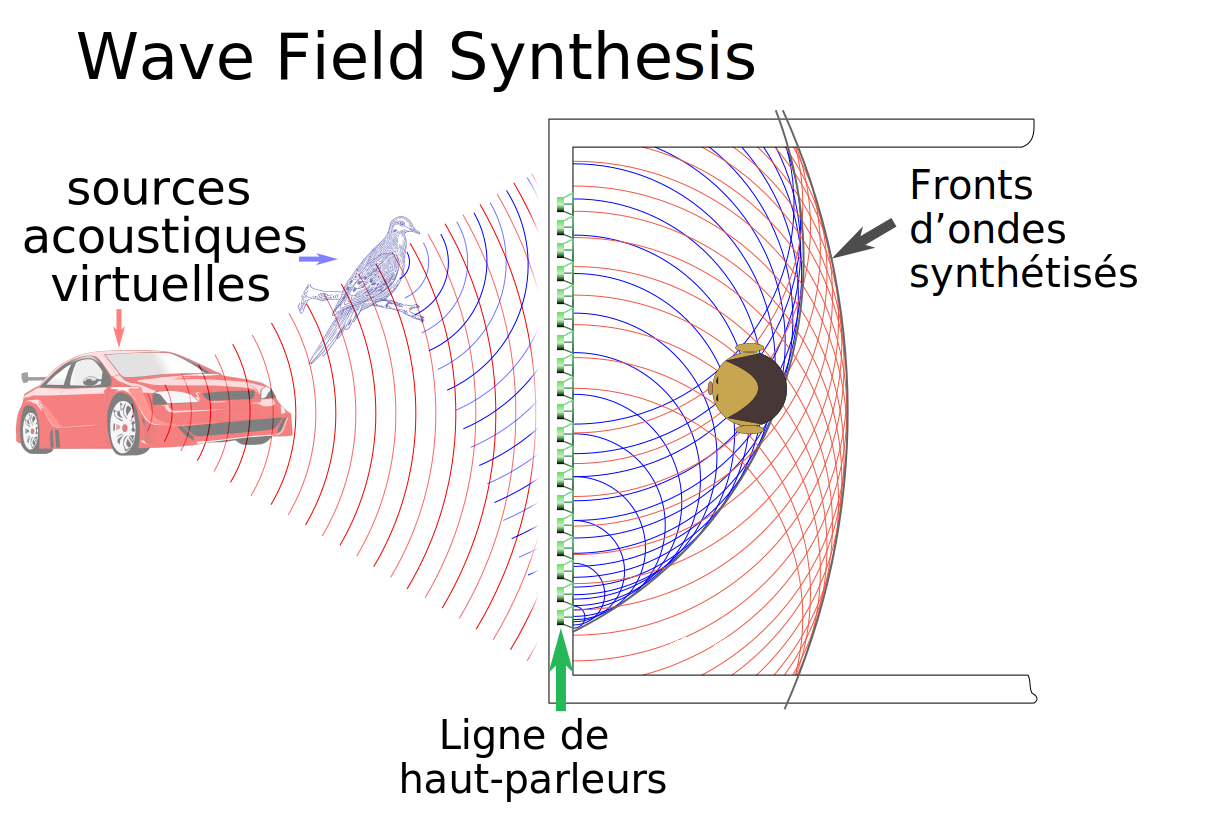
\includegraphics[width=1\linewidth]{./figures/ch2/wfs_edit.png}}
    \caption{}
    \label{Fig:wfs_edit}
  \hspace{0.3cm}
  \end{subfigure}
  \caption[(a) Illustration de la différence de fréquence et de niveau des ondes sonores interprétées par le cerveau suivant la localisation de leurs sources. (b) Schéma simplifié de la technique de Wave Field Synthesis.]{\it (a) Illustration de la différence de fréquence et de niveau des ondes sonores interprétées par le cerveau suivant la localisation de leurs sources. Source : \textit{2007 Thomson Higher Education}
  (b) Schéma simplifié de la technique de Wave Field Synthesis consistant à reproduire des vagues sonores complexes grâce à une ligne de haut-parleurs permettant de dissocier les sources sonores suivant leur nature et leur localisation. Source : \cite{www.syntheticwave.de.dove_english:_2015}
  }
  % \hspace{0.3cm}
\end{figure}

\subsection{Interaction}

Nous avons vu que les moyens dédiés à l'immersion sont nombreux et permettent de provoquer susciter chez le sujet au coeur de la scène virtuelle, faisant de lui un observateur actif autour des objet explorés dans le cas de la stéréoscopie adaptative.

Pour que le sujet puisse devenir l'acteur de ce monde virtuelle, il faut lui fournir
 possibilité d'interagir avec l'environnement virtuel ce qui assure par ailleurs une plus grande implication de l'utilisateur \cite{steuer1995defining}. Les techniques et méthodes d'interactions n'ont pas connu la même évolution rapide que les systèmes d'immersion et il est encore difficile de mettre en avant des techniques d'interactions opérationnelles dans tous les Environnements Virtuels (EV) et pour tous les contenus et tâches virtuels.

\subsubsection{Périphériques de tracking pour l'interaction} \label{peripheriques}

L'utilisation de périphériques de tracking pour interagir avec un EV immersif est la solution la plus communément utilisée au sein des EV immerifs. A la différence des moyens d'interaction en conditions classiques de bureau, les techniques de tracking sont adaptées à des conditions d'utilisation en position debout et dans des conditions d'obscurité. A l'aide de ces techniques, la souris des stations de travail a fait place à des périphériques tels que la souris 3d, appelée aussi \textit{Flystick} (cf Figure \ref{Fig:art_flystick}). Le \textit{Flystick} se caractérise par un périphérique à une main composé de boutons et dont les contrôles directionnels sont déportés sur un mini-joystick ou une \textit{tracking ball} manipulables au pouce. La manette reste un dispositif très utilisé du fait de sa courte courbe d'apprentissage due à sa démocratisation et également du fait de son nombre de commandes possibles important via ses nombreux boutons et combinaisons de bouton, mais est plutôt utilisée comme dispositif de contrôle de navigation, car ce dispositif n'est pas situé dans l'espace.

On retrouve également des dispositifs spécialisés reprenant la forme des outils qui sont censés être utilisé dans le monde virtuel permettant plus de réalisme dans l'interaction. Ces outils sont aussi suivis par des dispositifs de tracking optique permettant de les intégrer à travers leurs avatars dans les scènes virtuelles. Ces périphériques sont particulièrement utilisés dans des situations d'apprentissage à l'aide d'environnements virtuels.

\begin{figure}
  \centering
  {\includegraphics[width=.55\linewidth]{./figures/ch2/art_flystick}}
    \caption[Flystick, ou souris 3d.]{{\it Le Flystick2 d'ART, ou souris 3d, permettant d'interagir avec un environnement 3d en position fixe ou mobile.}}
  \label{Fig:art_flystick}
  \hspace{0.3cm}
\end{figure}

% Afin de se mouvoir et d'évoluer dans le monde virtuel, l'utilisateur doit pouvoir être positionné par la plateforme de rendu. La navigation dans un environnement virtuel est une problématique cruciale en RV, d'autant plus lorsqu'elle s'effectue au sein d'un environnement virtuel abstrait et en l'absence des repères spatiaux habituellement rencontrés dans le monde réel.
% Parmi les dispositifs permettant de récupérer les positions de la tête ou du corps de l'utilisateur, le \textit{tracking} optique est l'un des plus usités. Il fonctionne au moyen de caméras infrarouges et de marqueurs réfléchissants (voir Figure \ref{Fig:ir-tracking}). Des motifs de marqueurs vont servir de cibles pour les caméras infrarouges qui vont opérer une triangulation afin d'en extraire leur position. Chaque motif différent peut être associé à un objet particulier, une partie du corps ou un dispositif d'interaction. Le suivi de la tête est particulièrement utile dans les environnements immersifs puisqu'il permet de connaître la position et l’orientation de la tête et donc du regard au sein du monde virtuel. Grâce à cela, les ordinateurs responsables du rendu graphique peuvent adapter les images affichées sur les écrans pour qu'elle corresponde au point de vue de l'utilisateur dans le monde virtuel.
% Il est également commun d'utiliser le système de \textit{tracking} afin de capturer les gestes de la main afin de mettre en place des interactions précises avec l'environnement. L'interaction par capture peut également se faire au travers de dispositifs d'interaction de nature variée suivant l'activité exécutée en RV. Parmi ces outils spécifiques, la souris 3d également appelée \textit{flystick} ou la manette de jeu sont couramment utilisées dans les environnements immersifs.
% Enfin, il est possible de capturer l'ensemble du corps d'une personne afin de mettre en mouvement sa représentation virtuelle, appelée avatar. L'ensemble des marqueurs infrarouges va être réparti sur une combinaison afin d'obtenir la position de l'ensemble des parties mobiles du corps. Cette technique est beaucoup utilisée dans le monde du cinéma par exemple afin d'animer les avatars présents dans les films d'animation. Elle est également utilisée dans la recherche lorsque la perception de soi ou d'un collaborateur est importante pour la tâche à effectuer, par exemple au cours d'études ergonomiques.

% \begin{figure}
%   \centering
%   {\includegraphics[width=.65\linewidth]{./figures/ch2/IR-tracking}}
%     \caption{{\it Schéma simplifié d'un système de tracking optique basé sur des signaux infrarouges lancés par des caméras et se reflétant sur des marqueurs spécifiques. La configuration spatiale des marqueurs est reconnue par le PC et la position associée est calculée à partir des intersections de rayons infrarouges reflétés.}}
%   \label{Fig:ir-tracking}
%   \hspace{0.3cm}
% \end{figure}

\subsubsection{Interfaces sensori-motrices} \label{interface_sensor-motor}

 Ces interfaces regroupent les dispositifs permettant à la fois d'interagir avec l'environnement, mais également de recevoir un stimulus sensoriel en réponse. La plus commune des interfaces sensori-motrices est l'interface haptique qui va permettre à l'utilisateur de ressentir l'effet de son interaction. 

Les bras à retour d'efforts permettent par exemple de manipuler des objets en 3d tout en ressentant leur poids ou d'éventuelles collisions avec d'autres objets. Plus généralement, les systèmes à retour d'effort impliquent une plus grande précision des gestes et des manipulations de l'utilisateur.

Certains gants haptiques disposent de moteurs répartis sur l'ensemble de la main et des doigts permettant de faire ressentir à un utilisateur un objet particulier comme s'il l'attrapait réellement.

Le domaine médical et plus généralement des opérations télé-robotisées profitent de ces dispositifs afin de garantir un ressenti proprio-kinesthésique et tactile complémentaire à l'information visuelle. Ils sont courants en conception ou simulation de pilotages, car tentant de reproduire fidèlement les conditions réelles.
Dans les sciences, ils sont utilisés pour guider l'utilisateur à l'aide de retour de force lors des manipulations de systèmes moléculaires, afin de lui faire percevoir les forces en jeu dans la simulation du phénomène observé.

\subsubsection{Interactions gestuelles} \label{interface_nature}

Afin d'augmenter la sensation d'immersion de l'utilisateur et améliorer son expérience, il existe des interactions dites gestuelles qui vont chercher à s'inspirer des techniques.
Les interactions gestuelles, regroupant les interactions mettant en jeu des mouvements de l'utilisateur ou des commandes vocales pour interagir avec son environnement virtuel, font opposition aux interactions indirectes comme peuvent l'être le clavier, la souris ou les dispositifs d'interaction immersifs comme la souris 3d ou les manettes évoquées précédemment. Ces interactions induisent une présence moins importante des menus, peu compatible avec l'immersion. Il faut cependant noter que ces interactions ont souvent une courbe d'apprentissage plus longue que les interactions indirectes, avec une robustesse plus faible. Elles sont aussi moins contraignantes pour l'utilisateur puisqu'elles ne se basent pas sur une charge matérielle supplémentaire dans les mains de l'utilisateur autre que des supports de marqueurs pour la capture de gestes \cite{bossard2005gestural} et un micro, déporté ou non, pour la reconnaissance vocale. 

La combinaison des différentes méthodes d'interaction que nous avons vue est un domaine de recherche à part entière \cite{martin_hardware_2014,martin_reconfigurable_2011}. On parle de \textbf{multimodalité} lorsqu'on propose aux utilisateurs des interactions au travers de leurs différents canaux sensori-moteurs. Cette combinaison va permettre de gérer des actions complexes et complémentaires réduisant ainsi le besoin de simplification des tâches entre les versions non-immersive et immersive d'un programme.

\subsection{Navigation} \label{navigation}

La navigation dans un monde virtuel permet d'étendre les limites de l'immersion au-delà des contraintes physiques imposées par les dispositifs immersifs. C'est ce qui la distingue de la vision adaptative qui se restreint à ces limites physiques. 

\subsubsection{Définition}

La navigation est un concept qui nécessite une clarification terminologique, car comme le constatent Darken et Peterson, spécialistes en cognition spatiale, il existe une certaine confusion dans la littérature sur les termes employés \cite{darken2002spatial}. Ainsi, certains auteurs emploient comme synonyme les termes de « navigation », « déplacement » ou encore « exploration ». Ces trois termes sont utilisés tout trois dans notre étude d’où l’importance de définir clairement ces termes. La navigation dans des environnements réels ou virtuels se définit à la fois par des composantes \textbf{motrices} et à la fois par des composantes \textbf{cognitives} \cite{bowman_doug_a_3d_2002}.

\begin{itemize}
  \item La composante motrice définit le mouvement/déplacement réel d’un utilisateur dans l’espace. Il existe plusieurs modes ou techniques de déplacement. Bowman (2002) les classe en deux catégories, selon la métaphore employée pour se déplacer dans l’espace virtuel :
    \begin{itemize}
      \item Les métaphores réelles qui font appel à des comportements réalistes et/ou naturels comme le déplacement en mode « marche », « vol », « à vélo » ou encore « en conduisant ».
      \item Les métaphores « virtuelles » où les chercheurs utilisent le potentiel du virtuel pour imaginer et créer des métaphores pour permettre le déplacement dans l’espace.
    \end{itemize}
  \item La composante cognitive ou « wayfinding » est un processus cognitif de définition d’un chemin à travers un environnement. Le « wayfinding » a pour principal objectif de permettre au sujet de se construire une « carte cognitive » de l’espace exploré.
\end{itemize}

Dans un environnement virtuel, les utilisateurs peuvent disposer de plusieurs objectifs lors de l'activité de navigation. Trois tâches de navigation ont été identifiées par Darken et Sibert \cite{darken1996navigating} de façon générique alors que Van dam et al. \cite{van_dam_immersive_2000} ainsi que Bowman \cite{bowman_doug_a_3d_2002} en proposent une quatrième prenant tout son sens dans le cadre de la navigation pour la visualisation scientifique :

\begin{enumerate}
  \item  L'\textbf{exploration} c’est-à-dire une navigation sans cible explicite à atteindre. Le but étant uniquement de connaître et comprendre le nouvel environnement exploré. L’exploration peut aussi être psychologiquement active si le sujet doit suivre des indications. Dans le cas contraire, l’exploration est dite psychologiquement passive.
  \item La \textbf{recherche d'une cible inconnue} où le sujet cherche une cible/destination particulière mais ne connaît pas la position de celle-ci.
  \item La \textbf{recherche d'une cible dont la position est connue} dans lequel La tâche/objectif est de retrouver une cible.
  \item La \textbf{manoeuvre} consiste en des mouvements courts permettant à l'utilisateur de se positionner et de d'orienter.
\end{enumerate}


La dissociation entre les distances pouvant être parcourues dans un monde virtuel et les contraintes dimensionnelles des dispositifs immersifs a rapidement obligé les experts en RV de mettre au point des méthodes de navigation répondant à cette problématique. Ces méthodes ne répondent pas seulement au besoin de changement d'échelle entre l'espace réel d'interaction et l'espace virtuel de navigation, elles doivent également prendre en compte les effets induits par l'activité de navigatio,  notamment la une perte de repères spatiaux.  

Cette perte de repères spatiaux n'est pas le seul fait de paradigmes de navigation, elle sera également accentuée par le caractère abstrait et donc non écologique des données observées. Alors que la navigation au sein d'une ville ou d'une pièce peut permettre de garder pour le sujet une conscience de sa position et de son orientation suffisante, la navigation dans une scène représentant des informations abstraites et/ou non orientées diminuera cette capacité à savoir se situer par rapport au contenu et au monde virtuel. Les degrés de liberté de l'utilisateur pour naviguer dans sa scène virtuelle sont également un facteur pouvant compromettre sa bonne conscience spatiale. Alors que les scènes réalistes vont souvent induire une navigation avec 2 degrés de liberté parallèlement au sol virtuel, les scènes possédant des données abstraites nécessite une navigation en 3 dimensions dans l'ensemble du volume composant la scène virtuelle. 

La réduction ou l'absence de repères spatiaux n'a pas seulement une conséquence sur le fait qu'un utilisateur puisse se sentir perdu au milieu d'une scène virtuelle. Elles peuvent également déclencher ou favoriser l'apparition d'un sentiment de malaise, communément appelé \textit{cybersickness}, ou mal du simulateur. 

\subsubsection{Mal du simulateur ou \textit{cybersickness}} \label{cybersickness}

Le \textit{cybersickness} peut s'apparenter au mal des transports, transposé aux mondes virtuels, et se caractérisant par plusieurs effets indésirables et désagréables pour l'utilisateur. En plus de simples sensations d'inconfort, on retrouve comme symptômes de la fatigue excessive, des vertiges, des maux de tête ou des nausées, dégradant de manière importante la qualité de l'expérience de l'utilisateur \cite{kolasinski1995simulator,laviola_jr_discussion_2000}. Le mal du simulateur est susceptible de diminuer l'efficacité de l'utilisateur lors de l'éxécution de ses tâches et induit également un phénomène de rejet vis-à-vis du dispositif immersif. Ce phénomène fut donc étudié de près afin d'en identifier les causes et d'en trouver des solutions. Les causes principales mises en évidence lors des expériences de RV menées dans le but d'induire ce phénomène passent presque exclusivement par la dissociation des canaux perceptifs du corps humain. Le découplage et l'incohérence des informations fournies par canal visuel avec celles du système vestibulaire  est notamment identifié comme étant une cause probable du cybersickness \cite{reason1975motion}. 

Ainsi, une scène virtuelle impliquant un déplacement non contrôlé de l'utilisateur et dont les paramètres de vitesse, d'accélération et de rotations, entraîne dans beaucoup de cas le mal du simulateur. Ces situations de déplacements non contrôlés par l'utilisateur sont également identifiées comme responsables du mal des transports. L'absence d'implication d'un usager durant la navigation, peut également être un facteur déclencheur du cybersickness. Ce phénomène a été observé lors du visionnage de film ou de contenu vidéo impliquant des  déplacements non contrôlés par le sujet même sur un rendu non stéréoscopique. L'immersion sans contrôle amplifie le phénomène de cybersickness, effet observé lors du visonnage du film <<The Walk>>\footnote{\url{https://en.wikipedia.org/wiki/The\_Walk\_\%282015\_film\%29}}, sorti au cinéma en format 3D en septembre 2015, un nombre très significatif de personnes ayant rapporté souffrir de nausées et de vomissements \footnote{\url{http://www.theguardian.com/film/2015/sep/30/robert-zemeckis-3d-the-walk-audiences-vertigo}}. Il n'est cependant pas envisageable de réduire l'immersion afin de réduire le \textit{cybersickness}, il est donc important de jouer sur les facteurs impliqués dans le cybersickness est proposant des paradigmes de navigation qui permettent de minimiser le mal du simulateur.

%Le taux de rafraîchissement des images affichées, plus lent que la vitesse d'analyse du cerveau, peut créer un différentiel faisant apparaître des défauts dans l'espace d'affichage et ainsi participer à l'apparition d'un malaise. Ce défaut, principalement technique, s'explique par les ressources importantes demandées par les dispositifs immersifs et les contenus virtuels. Un taux de rafraîchissement supérieur à 40 images par seconde pour chacun des yeux (en cas de stéréoscopie active) n'est pas toujours atteignable pour les contenus virtuels complexes. 

%De nombreux efforts sont donc effectués pour réduire les temps de réponse et de latence des environnements immersifs afin de rapprocher l'expérience immersive de l'expérience réelle.

%Lors d'une immersion importante de l'utilisateur, ses attentes visuelles seront comparables à celles qu'il auraient dans le monde réel. Le passage d'un point de vue à un autre est donc une phase critique qu'il est nécessaire de contrôler et de rapprocher le plus possible d'une expérience réelle. La transition entre deux points de vue, si elle peut être instantanée, à la manière d'une téléportation, dans un environnement non-immersif, ne pourra qu'être perturbante dans un EV immersif. Il est donc important de mettre en place des changements de point de vue progressifs, dans l'idéal contrôlés par l'utilisateur, afin que celui-ci, en plus de ne pas perdre ses repères spatiaux, puisse anticiper et comprendre sa trajectoire.

%Parmi les autres pistes de solutions, nous avons vu qu'une incohérence de niveau de sollicitation du système vestibulaire de l'utilisateur par rapport à ce qu'il voit peut entraîner une augmentation de la probabilité de malaise. Augmenter l'implication corporelle de l'utilisateur pourrait donc constituer une réduction significative des risques d'apparition du \textit{cybersickness}. Cette augmentation de l'implication corporelle peut se faire à travers les paradigmes de navigation développés. Lorsque l'utilisateur est suivi par un système de \textit{tracking}, son corps et ses mouvements peuvent être interprétés afin de déclencher des mouvements dans le monde virtuel. Plusieurs techniques de navigation découlent du \textit{tracking} de gestes ou de position afin de diriger la navigation virtuelle.

Nous décrivons ci-dessous les différentes paradigmes de navigation, incluant ceux basées sur les technologies de \textit{tracking} et cherchant à répondre aux besoins d'exploration des mondes virtuels en prenant en compte les facteurs inhérents au phénomène de mal du simulateur.


\subsubsection{Navigation au sein de scènes virtuelles réalistes}

Il existe plusieurs degrés de contrôle de la navigation dans des environnements virtuels 3d, allant d'un contrôle absolu de l'utilisateur sur ses déplacements au sein de la scène virtuelle explorée à un calcul logiciel automatisé des chemins de navigation imposés à l'utilisateur en fonction du contenu virtuel.

\myparagraph{Navigation libre}

On regroupe dans ces méthodes les approches permettant à l'utilisateur de diriger ses déplacements au sein d'un EV. Ce contrôle peut passer par des techniques s'inspirant du contexte écologique, comme dans le cadre de technique mimant la marche, ou de techniques non écologiques caractérisées par des métaphores utilisant des dispositifs d'interaction tel que des manettes, des joysticks ou des souris 3d.

Pour mimer les conditions écologiques, on peut citer les \textbf{tapis roulants multidirectionnels} qui sont des dispositifs mécaniques permettant de simuler plusieurs actions physiques du monde réel dont la marche, la course, le fait de s'accroupir et parfois même de s'asseoir (voir Figure \ref{Fig:cyberith_virtualizer}). Leur fonctionnement est similaire aux tapis roulants standards mais la grande différence provient de leur capacité à bouger dans toutes les directions, offrant ainsi à l'utilisateur une possibilité de déplacement dans toute les direction en restant dans un espace de travail physique contraint. Cette technique permet également de libérer les mains de l'utilisateur de tout périphérique dédié à la navigation. Enfin, l'implication physique de l'utilisateur permet de réduire le phénomène de \textit{cybersickness} comme évoqué dans la section \ref{cybersickness}.
Ces périphériques se couplent aussi bien à des dispositifs immersifs type CAVE qu'à des dispositifs mobiles comme les HMD.

%Cependant, les développements les plus conséquents en RV sont passés par des techniques naturelles. 

\begin{figure}[h]
  \begin{subfigure}{.5\textwidth}
  \centering
  {\includegraphics[width=0.9\linewidth]{./figures/ch2/cyberith_virtualizer}}
    \caption{}
    \label{Fig:cyberith_virtualizer}
  % \hspace{0.3cm}
  \end{subfigure}
  \begin{subfigure}{.5\textwidth}
  \centering
  {\includegraphics[width=0.9\linewidth]{./figures/ch2/omnideck}}
    \caption{}
    \label{Fig:omnideck}
  \hspace{0.3cm}
  \end{subfigure}
  \caption[(a) Tapis roulant multidirectionnel statique (\textit{Cyberith Virtualizer}). (b) Premier tapis roulant multidirectionnel large et statique (\textit{Omnifinity Omnideck})]{\it (a) Tapis roulant multidirectionnel statique (\textit{Cyberith Virtualizer}) permettant de reconnaître, en plus de la marche et la course, des mouvements verticaux comme le saut ou l'accroupissement.
  (b) Premier tapis roulant multidirectionnel large et statique (\textit{Omnifinity Omnideck}), utilisé en couplage avec une technologie de \textit{tracking} optique afin de garantir un suivi précis des mouvements de l'utilisateur.
  }
  % \hspace{0.3cm}
\end{figure}

A l'opposé des paradigmes de navigation les plus écologiques, les techniques de navigation très bon marché et les plus communément usitées, basées sur des dispositifs d'interaction tels que des manettes et des joystick, inspirées des jeux vidéos, ne nécessitent pas une véritable implication physique du sujet. Cependant l'implication physique étant un facteur permettant de diminuer le cybersickness,

Pourtant, dans le cadre de casques virtuels, les dispositifs d'interaction, utilisables sans que l'utilisateur ait besoin de percevoir visuellement ses mains, sont pour l'instant privilégiés. 

De manière intermédiaire, d'autres techniques basées sur le \textit{tracking} nécessitent une implication du système vestibulaire de l'utilisateur. Cette implication étant un facteur permettant du \textit{cybersickness} elles constituent un bon compromis entre les techniques de navigation très réalistes mais très coûteuses et des techniques qui ne requiert pas d'implication physique.

\myparagraph{Navigation automatique ou semi-assistée}

La navigation automatique dans une scène virtuelle peut s'apparenter à une navigation dans un véhicule sur lequel l'utilisateur n'aurait aucun contrôle \cite{habibi20143d}. Cette navigation complètement automatique, où les déplacements de l'utilisateur seront dirigés par le programme, peut se faire selon deux méthodes principales :

\begin{itemize}
  \item Méthodes de \textit{\textbf{path finding}} : ces méthodes demandent la définition de points de passage dans la scène virtuelle. Ces points de passage, considérés comme les meilleurs points de vue, peuvent être définis manuellement ou automatiquement. En cas de définition automatique, on se servira de la nature de la scène à explorer afin de les définir. Plusieurs méthodes existent pour trouver les points singuliers de la scène. Certaines méthodes  se basent sur des analyses de l'entropie de la scène et cherchent les points de vue permettant de visualiser un maximum d'objets 3D en même temps\cite{vazquez2001viewpoint}. Il est également possible de se baser sur les informations lumineuses afin d'extraire les meilleurs points de vue . Dans ce cas là, ce seront les points de vue maximisant l'illumination de la scène qui seront retenus et constitueront les points de passage de la caméra pendant l'exploration automatique de la scène \cite{gumhold2002maximum}.
  \item Méthodes de contrôle \textbf{basées sur les images}: il est ici question de déplacer la caméra en optimisant une fonction de coût dont les paramètres sont définis en fonction des propriétés des images.  Ces approches sont particulièrement appropriée afin de suivre les modifications et des singularités de la scène, comme un objet en mouvement par exemple \cite{courty2001computer}. 
\end{itemize}

Dans une situation de navigation automatisée, la seule liberté de l'utilisateur est la direction de son regard, le \textit{tracking} de tête ou les informations du système gyroscopique associé au dispositif utilisé permettant de déterminer cette direction.

Il est également possible de mettre en place une navigation semi-assistée ou semi-contrôlée où cette fois l'utilisateur pourra contrôler une partie des paramètres de navigation. Parmi ces paramètres, soit la direction, la vitesse ou l'accélération seront le fait d'interactions de l'utilisateur, les autres paramètres étant dirigés par le programme. Il est ainsi possible de créer des chemins de navigation pré-calculés à partir d'une position de l'utilisateur, ce dernier devant choisir le chemin qu'il considère optimal pour sa tâche. A chaque nouvelle position, de nouveaux chemins optimaux seront calculés et soumis au choix de l'utilisateur.
Cela passe également par la mise en place de contraintes, soit d'orientation, soit de direction, ou encore de vitesse qui viendront influencer le déplacement de l'utilisateur vers un point donné ou autour d'un objet d'intérêt. Ces contraintes, lorsqu'elles sont mises en place, reflètent souvent la volonté de la part du créateur de la scène virtuelle de garder l'attention de l'utilisateur sur le coeur de sa tâche et de simplifier sa navigation pour qu'il se concentre sur l’exécution de cette tâche \cite{salomon2003interactive}.

\myparagraph{Paradigmes}

Au delà des périphériques d'interaction utilisé pour la navigation, les paradigmes permettant de traduire une commande issue de ces dispositifs par un déplacement dans le monde virtuel sont nombreux. Les professionnels du jeu vidéo conçoivent depuis longtemps des paradigmes de navigation variés et appliqués la plupart du temps à des contenus réalistes, 2d ou 3d, utilisant des dispositifs spécifiquement conçu pour un usage domestiques, comme les manettes ou les joystick.

Dans des domaines plus industriel, les paradigmes propres aux simulation de transports comme le vol ou la conduite de véhicule sont utilisés dans les scènes virtuelles constituées de grandes étendues à explorer (cf. Figure \ref{Fig:driving_simu}). Proches des conditions réelles de pilotage ou de conduite, ils permettent d'assurer une certaine identité de l'expérience réelle/virtuelle et possède une courbe d'apprentissage courte puisque basée sur l'expérience des utilisateurs.

\begin{figure}[h]
  \begin{subfigure}{.5\textwidth}
  \centering
  {\includegraphics[width=0.9\linewidth]{./figures/ch2/driving_simu}}
    \caption{}
    \label{Fig:driving_simu}
  % \hspace{0.3cm}
  \end{subfigure}
  \begin{subfigure}{.5\textwidth}
  \centering
  {\includegraphics[width=0.9\linewidth]{./figures/ch2/flight_simu}}
    \caption{}
    \label{Fig:flight_simu}
  \hspace{0.3cm}
  \end{subfigure}
  \caption[(a) Exemple d'un simulateur de vol. (b) Exemple d'un simulateur de conduite.]{\it(a) Simulateur de conduite dans un système de rétroprojection sur écran courbé.\footnote{\url{http://www.lexus-int.com/design/virtual-reality.html}
  (b) Exemple du simulateur de vol Birdly où les déplacements virtuels sont la conséquences des mouvements réels de l'utilisateur adoptant une posture de chute libre.}
  }
  % \hspace{0.3cm}
\end{figure}


En réalité virtuelle, au delà des approches qui tentent de reproduire de manière stricte un déplacement dans le monde réel, des paradigmes de navigation s'appuient sur le \textit{tracking} de tête ou du corps. Parmi ces approches, certaines considèrent chaque position de l'utilisateur par rapport à une zone spatiale de référence. Un déplacement dans la direction de la droite reliant la zone de référence à la position de l'utilisateur, à la manière d'un joystick où l'utilisateur serait le sommet du manche et la zone de référence constituerait la base de ce manche (voir Figure \ref{Fig:HCNAV}) \cite{Bourdot2002HCNav}.

\begin{figure}[h]
 \centering
 {\includegraphics[width=0.8\linewidth]{./figures/ch2/HCNav}}
   \caption[Technique de navigation HCNav.]{\it Exemple de l'utilisateur des déplacements relatifs d'un utilisateur par rapport à une zone de référence pour contrôler son déplacement dans le monde virtuel. L'orientation de son regard décidera également des rotations dans le monde virtuel. Il est donc possible d'avoir un contrôle de 6 degrés de liberté pour la navigation (3 en translation et 3 en rotation).}
   \label{Fig:HCNAV}
 \hspace{0.3cm}
\end{figure}

Le \textit{tracking} des mouvements de l'utilisateur est aussi utilisé afin de traduire le mouvement naturel de la marche en un équivalent dans le monde virtuel. 

D'autres techniques plus avancées comme la \textbf{marche redirigée} exploitent l'imprécision chez l'homme de la perception de la rotation de sa tête, pour induire une trajectoire courbe de son déplacement physique pour le contraindre dans espace de travail physique restreint, alors que le sujet a l'impression de marcher en ligne droite dans le monde virtuel \cite{bruder_redirecting_2012}.

Il existe donc une large variété de paradigmes permettant l'exploration et la navigation au sein de scènes écologiques. 




\section{Apports et usages de la réalité virtuelle en biologie structurale} \label{RV_for_bio_struct}

La RV possède plusieurs facettes répondant naturellement aux problèmes posés par l'analyse scientifique. Rappelons la problématique actuelle de la visualisation de données scientifiques. Les données générées excèdent de loin les capacités d'interprétation humaines. De plus, la complexité et la quantité des données sont telles que leur rendu 2D ou 3d sur des écrans d'ordinateur ne sont plus suffisants pour rapporter l'ensemble des informations que les données contiennent. %L'accès à certaines informations est donc entravé et enfoui sous la quantité de données à analyser par l'utilisateur.

\subsection{L'immersion dédiée à la visualisation moléculaire}

Dans le cadre de la visualisation scientifique, on peut considérer que la capacité d'affichage stéréoscopique doublée à une surface d'affichage à 360 degrés est la caractéristiques qui la rend la plus attractive pour l'exploration de données scientifiques. Plusieurs études ont par exemple démontré que la perception de la profondeur lors de la représentation de structures moléculaires apportait une aide non négligeable pour leur compréhension structurelle \cite{van_dam_immersive_2000,stone_immersive_2010,odonoghue_visualization_2010}. Les complexes moléculaires et les protéines sont par nature structurés en 3d et c'est cette structuration qui est au cœur des études en biologie structurale. La stéréoscopie s'est donc imposée comme une techniques adaptée pour l'observation de structures protéiques. 
Mais l'étude de la structure seule ne peut suffire lors de l'étude d'un complexe moléculaire, nous avons souligné auparavant la présence de nombreuses données accompagnant la génération de modèles 3d lors d'une simulation moléculaire. 

%Ces données, sous forme de valeurs brutes, doivent être également analysées. La dimension de profondeur propre à la stéréoscopie prend une nouvelle fois tout son sens ici. Ce n'est plus la nature 3d même des données observées qui va rendre cette profondeur importante, puisque nous nous intéressons maintenant à des valeurs numériques brutes, mais la possibilité d'utiliser une 3e dimension pour représenter des modèles, des tendances ou bien des anomalies au sein des données affichées.

%Au-delà de la stéréoscopie, la surface, ou davantage le volume quand on parle de 3d, disponible dans les dispositifs de RV pour afficher des informations est beaucoup plus important que ce qu'on peut retrouver au sein de dispositifs 2d standards. Combiné avec un suivi de l'orientation et de la position de la tête de l'utilisateur, il devient aisé de créer un monde composé de 360 degrés d'informations accessibles simplement et rapidement au moyen d'un simple coup d'œil.

\subsection{Les interactions multimodales}

%La notion d'interaction n'intervient pas que dans un sens unique et même si la méthode permettant d'interagir avec un objet est primordiale, le retour sensoriel provoqué par l'interaction est, en RV, un sujet d'étude à part entière. 

Nous avons vu que ces retours sensoriels participent à l'immersion ressentie par l'utilisateur dans un monde virtuel, mais ils peuvent également servir de repères ou de vecteurs d'informations utilisés pour compléter les informations visuelles. Même s'il est possible de mettre en place certaines sollicitations autres que visuelles lors d'un travail sur un poste de travail standard, il est très rare de trouver des retours sonores ou haptiques lors d'une session de travail. Au-delà des limites matérielles qui peuvent exister, un retour haptique impliquant par exemple la nécessité de posséder un dispositif muni d'un système de retour d'effort, les limites sont souvent logicielles. Peu de programmes implémentent des retours sensoriels autres que visuels dans la conception de leurs outils d'analyses de données. Il est au contraire très commun de prendre en compte ces retours sensoriels lors du développement de solutions logicielles dédiées à la RV. 

La RV est par essence définie par l'implication de l'utilisateur. Elle a donc dû développer très tôt des moyens pour retranscrire un maximum de sensations aux utilisateurs lors de leurs expériences virtuelles. Les systèmes haptiques ont su rapidement venir de la RV jusqu'aux laboratoires de biologie structurale dans le but permanent d'améliorer la perception 3d des structures moléculaires d'intérêt. La possibilité de toucher une molécule, en combinaison de sa visualisation 3d, offre une complémentarité importante pour la compréhension de certaines particularités structurelles \cite{stocks2009interacting}.

Le domaine du docking moléculaire fut assez friand de la technologie de bras haptique afin de permettre le ressenti des forces d'interaction prenant place entre deux partenaires \cite{nagata2002concept, sankaranarayanan2003role}. L'ajout de la flexibilité dans les techniques de docking et l'utilisation de techniques de simulations interactives (voir section \ref{simu_interactive}) où des forces peuvent être ajoutées par l'utilisateur au sein d'une simulation en cours fut aussi un terrain propice à l'utilisation de systèmes de retours haptiques \cite{stone2001system}. Ces derniers permettent en effet un contrôle fin de la force appliquée et imposent une limite physique à celle-ci que l'utilisateur ne peut dépasser. Le matériel a pu évoluer avec le temps afin de répondre aux besoins évoluant des équipes de recherche et un aperçu de cette évolution est illustrée dans la Figure \ref{Fig:taylor_haptic}.

\begin{figure}[h]
  \begin{subfigure}{.3\textwidth}
  \centering
  {\includegraphics[width=0.95\linewidth]{./figures/ch2/taylor_haptic}}
    \caption{}
    \label{Fig:taylor_haptic}
  % \hspace{0.3cm}
  \end{subfigure}
  \begin{subfigure}{.34\textwidth}
  \centering
  {\includegraphics[width=0.98\linewidth]{./figures/ch2/haptic_docking}}
    \caption{}
    \label{Fig:haptic_docking}
  % \hspace{0.3cm}
  \end{subfigure}
  \begin{subfigure}{.34\textwidth}
  \centering
  {\includegraphics[width=0.98\linewidth]{./figures/ch2/ferey_haptic}}
    \caption{}
    \label{Fig:ferey_haptic}
  % \hspace{0.3cm}
  \end{subfigure}
  \caption[Système haptique \textit{the Docker}. (b) Système haptique Phantom. (c) Système haptique permettant la manipulation d'une protéine.]{\it (a) Système haptique appelé \textit{the Docker} conçu et construit par Ming Ouh-young et permettant de simuler les forces et les torsions dues aux interactions électrostatiques entre les deux molécules.
  (b) Système haptique Phantom utilisé dans la salle immersive d'un laboratoire de réalité virtuelle dans le cadre d'une expérience mettant en jeu le contrôle d'un docking par interaction haptique. 
  (c) Système haptique permettant la manipulation d'une protéine au sein d'un laboratoire de biologie structurale dans le cadre d'une expérience de simulation moléculaire interactive (voir section \ref{simu_interactive}).
  }
  % \hspace{0.3cm}
\end{figure}

En visualisation de données abstraites et/ou scientifiques, l'utilisation  de retours sensoriels a donc pu être détournée de son but premier, l'immersion, pour communiquer des informations supplémentaires à l'utilisateur pendant ses phases d'interactions. La possibilité par exemple de déclencher un événement sonore lors de la sélection de données critiques ou extrêmes dans un set de données est l'un des exemples de l'utilisation d'un retour auditif pour transmettre une information \cite{ferey_multisensory_2009}. De la même façon, le domaine de la conception assistée par ordinateur (CAO), très présent en RV, utilise des dispositifs de retour de force afin de juger de la résistance de matériaux ou de limites de torsion/translation des objets \cite{sun2010haptic}. La chirurgie est également demandeuse de solutions précises de retours haptiques au sein de ses récentes applications de RV dédiées à l’entraînement des chirurgiens à des opérations spécifiques ou développées pour le contrôle de robots pour des opérations sur des patients réels \cite{kusumoto_application_2006}. Étendre ces moyens de fournir des informations par d'autres canaux que les canaux visuels pour la visualisation de données scientifiques en RV est donc une solution réaliste et concrète, simplifiée par les méthodes de RV déjà existantes.

\subsection{Interface moléculaire tangible et réalité augmentée}

Nous avons vu dans le chapitre précédent la place majeure qu'avaient les modèles physiques comme moyens de représentation en premier lieu, les représentations par ordinateurs ne permettant pas au départ une complexité équivalente aux modèles physiques, puis comme moyens de communications, moyens les plus simples à transporter et présenter lors de congrès. Désormais, plusieurs études considèrent leur utilisation comme vecteurs d'interaction. Ces études s'appuient sur l'évolution conjointe des techniques de Réalité Augmentée (RA) et d'impression 3d. 

Avant tout approfondissement des cas d'usages de ces modèles physiques, nous revenons rapidement sur les concepts de Réalité Augmentée et d'impression 3d. La RA se définit comme l'ajout en temps réel de contenus virtuels 2d ou 3d au sein du monde réel grâce à un dispositif informatique (smartphone, casques de RV, lunettes de RA). De nombreuses applications de la RA existent, du rendu de meubles virtuels dans des pièces d'habitation aux labels flottants d'information sur certains lieux touristiques. 
L'impression 3d est quant à elle une technologie permettant de fabriquer des objets à partir de leur modèle 3d informatique. 

Combinées ensemble, ces techniques permettent par exemple, après la conception et l'impression d'un modèle physique de protéine, son traitement visuel en temps réel pour le suivre (par \textit{tracking} de marqueurs spécifiques ou \textit{tracking} de forme/couleurs) et permettre un rendu visuel du modèle et l'affichage de propriétés ou d'informations de façon dynamique et toujours en temps réel \cite{gillet2005tangible}. 
Les modèles physiques de protéine peuvent être des modèles statiques monobloc mais peuvent aussi être des modèles physiques complexes et résultats d'assemblages de sous-unités physiques faisant l'analogie des acides aminés. Au-delà de la simple analogie, ce découpage permet de mettre en place des solutions techniques visant à imiter les énergies rotationnelles inter-acides aminés à l'échelle des sous-unités physiques \cite{chakraborty2013coarse}. Ces modèles physiques avancés peuvent être envisagés comme moyens d'interactions pour la reconstruction assistée de peptides ou l'estimation d'énergie potentielle \cite{martinez2015virtual}. Leurs changements conformationnels de modèles informatiques 3d simulés seraient induits par les déformations du modèle physique manipulé (voir Figure \ref{Fig:tangible_xav}).

\begin{figure}[h]
  \begin{subfigure}{.4\textwidth}
  \centering
  {\includegraphics[width=0.9\linewidth]{./figures/ch2/tangible_marker}}
    \caption{}
    \label{Fig:tangible_marker}
  % \hspace{0.3cm}
  \end{subfigure}
  \begin{subfigure}{.6\textwidth}
  \centering
  {\includegraphics[width=\linewidth]{./figures/ch2/tangible_xav}}
    \caption{}
    \label{Fig:tangible_xav}
  \hspace{0.3cm}
  \end{subfigure}
  \caption[(a) Système de Réalité Augmentée grâce à des modèles tangibles de protéines. (b) Reconstruction 3d d'un modèle à partir d'un modèle physique complexe.]
  {\it (a) Tracking par marqueurs de modèles monobloc de protéines et rendu vidéo en réalité augmentée ajoutant les résidus chargés en bleu et rouge. Travail effectué au sein du <<Olson Laboratory>>.\footnote{\url{http://mgl.scripps.edu/}}
  (b) Reconstruction 3d d'un modèle complexe de peptide formé de groupes physiques distincts et possédant des aimants afin de rapporter les forces rotationnelles de liaison grâce à un retour haptique. Un rendu temps réel est effectué en parallèle grâce à un tracking par analyses d'image. Travail effectué au sein de VENISE, groupe du LIMSI-CNRS.
  }
  % \hspace{0.3cm}
\end{figure}


\subsection{Simulation moléculaire interactive} \label{simu_interactive}

Certaines simulations moléculaires, couplées à de rendus graphiques très performants et des dispositifs d'interactions 3d, permettent à l'utilisateur de contraindre certaines parties d'une structure moléculaire pendant sa simulation en injectant dans les calculs physiques des forces s'appliquant sur les particules manipulées \cite{bolopion_comparing_2010}. Le jeu sérieux Foldit\footnote{\url{https://fold.it/portal/}} s'appuie sur les stratégies et l'esprit d'analyse des utilisateurs, experts ou non du domaine, pour guider les changements conformationnels de protéines par des commandes simples. Un score est calculé en temps réel permettant de rendre compte de la stabilité énergétique de la structure obtenue. Alors que le chemin énergétique suivi par un algorithme standard va favoriser les changements conformationnels peu coûteux, l'esprit humain est capable d'anticiper un changement qui va contraindre la protéine de façon importante, mais permettant d'obtenir une structure plus stable par la suite \cite{khatib2011crystal}.

Il est également possible de générer des représentations volumiques de certaines informations expérimentales comme des cartes de densité de données cristallographiques ou SAXS afin de permettre à l'utilisateur d'agir sur les domaines flexibles de sa protéine afin de la faire entrer dans ces volumes. Certains travaux utilisent même directement l'aide de l'utilisateur afin de replier une protéine représentée grâce à des paramètres de mécanique moléculaire et déplacée/orientée dans une carte de densité électronique SAXS \cite{molza2014innovative}.

La possibilité d'influer ainsi sur une simulation moléculaire demande la mise en place d'une structure logicielle de haute performance, car des modules de simulation, de  visualisation, d'interactions homme-machine doivent fonctionner de façon synchronisée.
La représentation simplifiée de la protéine permet une certaine rapidité de la simulation et donc la prise en compte rapide de l'effet des changements opérés par l'utilisateur. Dans cette optique, le projet BioSpring permet la représentation de protéines par des réseaux de ressorts pour les interactions liées et des paramètres de champ de force configurables pour les interactions non liées \cite{ferey2012biospring}. Cette représentation semi-simplifiée permet de contraindre les parties rigides de la protéine tout en assurant une certaine flexibilité au niveau des régions moins structurées (boucles et coudes).

Dans le cas de dynamiques moléculaires sur des systèmes de taille plus importante, calculées dans des clusters de calcul déportés, les défis sont autres. Ils passent par la mise en place de communications privilégiées entre le centre de calcul et le lieu de visualisation et d'interaction. %En plus des communications, la précision demandée peut être supérieure et les forces appliquées au système doivent pouvoir être interprétées de façon instantanée par le programme de simulation. 
Des suites logicielles performantes permettent aujourd'hui de traiter une simulation de façon interactive alors même que cette dernière est déportée \cite{dreher2014exaviz}, à l'aide d'approche de  synchronisation et de parallèlisation très avancées compatibles avec le calcul haute performance. %Basée sur les principes de parallélisation d'instructions et d'utilisation des infrastructures de communications récentes offrant des vitesses de transmission de données au-delà de 10Gbit/s.


\subsection{Outils et applications}

La biologie structurale n'a su que tardivement se placer par rapport à l'immersion apportée par la RV. Si elle a utilisé certains de ses outils (systèmes haptiques par exemple), ce n'est que très récemment que certains programmes dédiés à l'exploration moléculaire ont commencé à être utilisés au sein de dispositifs immersifs de RV
% \commentaire{NF:je ne suis pas d'accord la biomol a su très tot intégrer des éléments de la réalité virtuelle, mais effectivement pas dans un cadre immersif}
\cite{odonoghue_visualization_2010}.

\commentaire{MB:Es-tu sur pour Yasara? Premiere fois que j'entends qu'il tourne en immersif/CAVE; un setup Desktop est certes possible, mais assez limite. } 
\correction{MT: Je dois avouer que je me suis référé à ça : http://www.yasara.org/products.htm\#cave}

YASARA \cite{krieger2014yasara} ou VMD \cite{stone_immersive_2010} sont deux exemples de programmes de visualisation moléculaires disponibles pour un rendu stéréoscopique et adapté aux environnements immersifs. Ils permettent l'interfaçage de leur solution de visualisation avec de nombreuses librairies utilisées en RV dans les systèmes immersifs de type CAVE ou mur d'écran. Parmi ces librairies, nous pouvons citer VRPN \cite{taylor2001vrpn}, FreeVR \cite{pape2004commodity} ou VR Juggler par exemple.

D'autres initiatives ponctuelles ont aussi vu le portage d'autres logiciels dans des environnements immersifs, mais ces développements spécifiques ont rarement dépassé l'extension du rendu graphique depuis le 2d jusqu'en 3d\footnote{\url{http://www.rug.nl/science-and-society/centre-for-information-technology/research/hpcv/vr\_visualisation/mol\_visualisation?lang=en}} ou la mise en place de librairies comme base de développement d'applications RV pour la visualisation moléculaire \cite{salvadori_moka:_2014}.  Afin d'améliorer l'apprentissage de certains concepts biologiques, il est parfois utile d'en améliorer la perception, en particulier quand ces concepts sont par certains aspects abstraits. Un projet éducatif a cherché à évaluer l'impact pour les étudiants de visualiser des objets moléculaires en RV dans le cadre de cours de biologie structurale \cite{tan_use_2013}. Selon leurs conclusions, les dispositifs immersifs ont permis un meilleur apprentissage des notions abordées ainsi qu'une compréhension globale plus complètede la biologie structurale.

L'usage des contextes immersifs dans le cadre de la biologie structurale est donc limitée et présente des pistes d'améliorations notables exposées ci-dessous.

%Le travail d'ingénierie est par aspects déjà fait, mais il semble manquer une réflexion ergonomique autour de l'intégration des outils de biologie structurale au sein de dispositifs immersifs.


\section{Limites et perspectives en Réalité Virtuelle pour la Biologie Structurale} % (fold)
\label{sec:RV_perspectives}

Nous avons dessiné dans la section \ref{RV_science} les contours de la RV et mis en avant les apports de son utilisation pour la biologie structurale dans la section \ref{RV_for_bio_struct}. 

%Au-delà des aspects immersifs qui la caractérisent, on retrouve la notion d'interaction adaptées et pertinentes pour la tâche de l'expert et au contenu qu'il manipule.

%Parmi les problématiques soulevées par la RV pour les données abstraites et scientifiques, nous avons évoqué que l'utilisation de la RV en biologie structurale etaient limité à des tâches d'exploration et de visualisation de structures 3d \commentaire{NF Quand?}. La réalisation de tâches nécessitant une interaction avec les données mises en jeu, dans un premier temps exclusivement 3d, nécessite la mise en place de méthodes de navigation adaptées. 
%Or la navigation au sein des mondes virtuels est l'un des obstacles cruciaux à franchir pour assurer une expérience optimale aux utilisateurs. 

La notion de monde virtuel implique la possibilité pour l'utilisateur d'évoluer au sein d'un environnement étendu de la même manière qu'il évoluerait dans la vie réelle. Or, si cette navigation virtuelle peut être inspirée de paradigme utilisé dans un cadre de navigation réelle dans le cas d'environnements virtuels écologiques, là où le contenu virtuel proposé est une copie artificielle d'éléments réels, la question est tout autre lorsque la scène observée n'est plus écologique et implique des éléments abstraits. 

%\subsection{Méthodes de navigation dans des scènes virtuelles abstraites}

Conçus autour de contenus réalistes, les paradigmes cités précédemment ne sont pas nécessairement transposables à des scènes abstraites. Leur efficacité est limitée du fait de la nature très différentes des données à observer. Alors que la navigation aura tendance à permettre l'exploration d'une surface virtuelle horizontale étendue dans des scènes réalistes, les scènes abstraites scientifiques, et plus particulièrement les scènes moléculaires, concentrent les informations dans une zone centrale autour de laquelle l'utilisateur va évoluer. L'échelle de visualisation des données est capable d'augmenter la distance (toujours à l'échelle) des données observées mais la nature même de l'exploration est souvent différente. Sheidermann décrit la visualisation de données comme un processus où l'exploration est l'étape préliminaire avant les étapes de zoom et de filtre qui précèdent elle-même l'étape finale de l'obtention des détails à la demande \cite{shneiderman_eyes_1996}. Les différentes échelles de précision mises en avant dans cette description sont rarement retrouvées dans les paradigmes de navigation au sein de scènes virtuelles réalistes.

Bien qu'il existe de nombreux portages de logiciels experts de visualisation moléculaire dans des EV, la navigation au sein de données scientifiques dans ces derniers s’inspire encore largement de la manipulation d'objet retrouvé dans les logiciels de visualisation moléculaire courants (voir Figure \ref{Fig:pymol_nav}) \cite{frohlich1999exploring}. Les seules tâches de navigation pouvant être identifiées au sein de logiciels experts de visualisation moléculaire se rapporte à des transitions progressives permettant de rejoindre une position spécifique depuis la position actuelle de l'utilisateur. Enfin, ces logiciels ne présentent aucune adaptation de la manipulation suivant le type de molécule observé et les paradigmes mis en jeu sont identiques, que l'objet observé soit une protéine de quelques acides aminés ou un virus de plusieurs millions d'atomes.

Ils permettent une navigation totalement libre autour de la molécule et n'imposent aucune contrainte, au détriment de la conscience spatiale de l'utilisateur. %La manipulation d'objets n'est cependant pas adaptée aux environnements virtuels. Le nombre et la complexité des tâches de manipulation sont trop nombreuses pour s'adapter aux EV immersifs qui favorisent des paradigmes de navigation simplifiées. 
La visualisation moléculaire met en scène des représentations artificielles d'atomes, non observables à l’œil humain en temps normal, et dont les couleurs et formes respectent des standards décidés par le domaine, non dictés par des observations réelles. Les repères spatiaux sont donc peu nombreux et souvent trop sommaires pour assurer une orientation acceptable de l'utilisateur. Ils se limitent donc au seul objet intérêt, son environnement (skybox, paysage, etc.) étant majoritairement vide avec un arrière-plan de couleur unie.   
 

\begin{figure}[h]
  \begin{subfigure}{.5\textwidth}
  \centering
  {\includegraphics[width=0.9\linewidth]{./figures/ch2/pymol_nav}}
  % \hspace{0.3cm}
  % \caption{}
  \label{Fig:pymol_nav}
  \end{subfigure}
  \begin{subfigure}{.5\textwidth}
  \centering
  {\includegraphics[width=\linewidth]{./figures/ch2/vmd_nav}}
  % \hspace{0.3cm}
  % \caption{}
  \label{Fig:vmd_nav}
  \end{subfigure}
  \caption[Captures d'écran des menus de navigation au sein de PyMol et VMD.]{\it Capture d'écran des interfaces de manipulation offerts par PyMol (à gauche) et VMD à droite. Ils sont constitués de nombreuses combinaisons souris/clavier pour permettre d'utiliser l'ensemble des possibilités de manipulation disponibles.
  }
  % \hspace{0.3cm}
\end{figure}


Le caractère abstrait des objets de la biologie structurale, décidera directement de la qualité de repères spatiaux que l'utilisateur possédera pour naviguer. Afin de combler ce manque préjudiciable pour l'expérience utilisatrice lors de ses futures tâches en biologie structurale, nous avons développé une série de paradigmes de navigation, basées sur le contenu observé et les tâches usuelles en visualisation/exploration moléculaire.

Dans la même optique de mettre en place un environnement virtuel respectant les contraintes de la RV, il nous a paru important d'adapter les interactions habituelles qu'un expert peut avoir dans des sessions de visualisation et d'analyses. Ces interactions, trop complexes et trop cloisonnées dans des environnements de bureau, doivent être simplifiées et harmonisées afin de pouvoir faire cohabiter et communiquer les étapes complémentaires que sont la visualisation et l'analyse. %On remarque que dans la boucle de la VA (voir Figure \ref{Fig:visual_analytics_process_keim}), ces deux étapes sont couplées de manière très étroites proches, aussi bien en terme de données utilisées que d'implication de l'utilisateur. Leur rapprochement et fusion au sein d'un unique module est pertinent et pourrait donc se faire à travers la mise en place d'une représentation des notions utilisées dans chacune des étapes. L'utilisation d'ontologie comme illustrée précédemment permet cela et va même plus loin, car elle pourrait simplifier l'étape de \textit{transformation} des données en imposant un carcan et un vocabulaire précis aux données d'entrée. Ce deuxième pan de notre étude nous a menés à la mise en place d'une plateforme multi-composants s'appuyant sur l'utilisation d'une base de données RDF (Resource Description Framework) dont la structure dépend directement d'une ontologie OWL (Web Ontology Language) créée pour décrire notre domaine d'application.

%Comme nous l'avons souligné auparavant, la génération de données de plus en plus complexes et de plus en plus massives produite de manière expérimentales ou théorique, pose de nombreux problèmes dans les étapes suivantes, notamment en terme de visualisation et d'analyse, et d'interprétation systématique des résultats produits. 

%Lors de l'étape de modélisation, les systèmes que l'expert doit construire en amont de l'étape de simulation sont de plus en plus complexe, nécessite la manipulation dans l'espace de nombreux acteurs.

%Il convient de mettre en place de nouvelles approches pour outiller ces usages, en couplant notamment plus étroitement les processus de production de données au processus d'interprétation d'analyse des données. 



% section probl_matique (end)